
\subsection{Дифференциал гладкого отображения}


\begin{definition}
	Пусть $M$ -- гладкое многообразие и $f : M \to \R^l$ -- гладкое отображение. \textit{Дифференциал} $df_p : T_p M \to \R^l$ 
	определяется так: для $v \in T_p M$ выберем соответствующую гладкую кривую $\gamma : (-\delta, \delta) \to M$ с $\gamma(0) = p$, $\gamma'(0) = v$, и положим 
	\[ df_p (v) := \frac{d}{dt} f(\gamma(t)) \Big|_{t=0} \tag{$*$} \]
\end{definition}

\begin{theorem}
	Пусть $M$ -- гладкое $m$-мерное многообразие и задано гладкое отображение $f : M \to \R^l$, где $p \in M$. 
	Справедливы следующие утверждения:
	\begin{enumerate}[itemsep = 0pt, topsep = 5pt]
		\item Правая часть $(*)$ не зависит от выбора $\gamma$,
		\item Отображение $df_p : T_p M \to \R^l$ линейно,
		\item Если $N$ -- гладкое многообразие в $\R^l$ и $f(M) \subset N$, то $df_p(T_p M) \subset T_q N$, где $q = f(p)$.
	\end{enumerate}
\end{theorem}

\begin{myproof}
	Пусть $v \in T_p M$. Выберем гладкую кривую $\gamma : (-\delta, \delta) \to M$, 
	такую что $\gamma(0) = p$, $\gamma'(0) = v$. 
	Рассмотрим гладкое продолжение $F : U \to \R^l$ функции $f$ в некоторую окрестность $U \subset \R^n$ точки $p$.
	Обозначим через $DF(p)$ матрицу Якоби $F$ в точке $p$. Так как $\gamma(t) \in M \cap U$ при малых $t$ по модулю, то 
	\[ DF(p) \cdot v = DF(\gamma(0)) \cdot \gamma'(0) = \frac{d}{dt} \Big|_{t=0} F(\gamma(t)) = \frac{d}{dt} \Big|_{t=0} f(\gamma(t)). \]
	Первое выражение в цепочке равенств не зависит от выбора $\gamma$, а последнее -- от выбора $F$. Это доказывает первый пункт.

	\vspace{5pt}
	Линейность отображения следует из полученного равенства $df_p(v) = DF(p) \cdot v$.

	\vspace{5pt}
	Если кривая $\gamma : (-\delta, \delta) \to M$ гладкая, $\gamma(0) = p$, $\gamma'(0) = v$, то 
	$\beta := f \circ \gamma : (-\delta, \delta) \to N$ тоже гладкая кривая, $\beta(0) = f(p) = q$, $\beta'(0) = df_p (v)$.
	Следовательно, $df_p (v) \in T_q N$.
\end{myproof}

\begin{corollary}
	Если в третьем пункте дополнительно дано гладкое отображение $g : N \to \R^s$, то справедливо цепное правило 
	$d(g \circ f)_p = dg_{f(p)} \circ df_p$.
\end{corollary}

\begin{myproof}
	Зафиксируем $v \in T_p M$, тогда $d(g \circ f)_p (v) = \frac{d}{dt} g(f(\gamma(t))) \big|_{t=0}$ для некоторой $\gamma$ из определения $v$.
	С другой стороны, $df_p(v) = \frac{d}{dt} f(\gamma(t)) \big|_{t=0} =: w \in T_q N$ и для кривой $\beta$ из доказательства третьего пункта имеем $d g_{f(p)} (w) = \frac{d}{dt} g(\beta(t)) \big|_{t=0} = \frac{d}{dt} g(f(\gamma(t))) \big|_{t=0}$, что совпадает с дифференциалом композиции.
\end{myproof}

\begin{corollary}
	Пусть $M$ -- гладкое $m$-мерное многообразие, $N$ -- гладкое $r$-мерное многообразие. 
	Если $f : M \to N$ является диффеоморфизмом, то $m = r$.
\end{corollary}

\begin{myproof}
	Пусть $p \in M$ и $q = f(p) \in N$. 
	Обозначим $g = f^{-1} : N \to M$. 
	Тогда $g \circ f = \id_M$ и $f \circ g = \id_N$, откуда по цепному правилу имеем
	$dg_q \circ df_p = \id : T_p M \to T_p M$ и $df_p \circ dg_q = \id : T_q N \to T_q N$.
	Следовательно, $df_p : T_p M \to T_q N$ является линейным изоморфизмом с $[df_p]^{-1} = dg_q$ и $m = \dim T_p M = \dim T_q N = r$, что и требовалось.
\end{myproof}

\begin{note}
	Из полученного следствия вытекает, что определение <<размерности>> гладкого многообразия корректно, то есть не зависит от выбора локальной параметризации.
\end{note}

\begin{note}
	Пусть $\phi : V \to \R^n$ локальная параметризация $M$ в окрестности $p = \phi(a)$, $v \in T_p M$ и $d \phi_a (h) = v$, тогда 
	$df_p (v) = df_p (d \phi_a (h)) = d (f \circ \phi)_a (h)$. В частности, 
	в координатах $df_p$ задается матрицей Якоби координатного представления $f \circ \phi$. 
\end{note}

\begin{definition}
	Пусть $f : M \to N$ -- гладкое отображение многообразия $M$ в многообразие $N$.
	Точка $q \in N$ называется \textit{регулярным значением} $f$, если дифференциал $df_p : T_p M \to T_q N$ сюръективен $\forall p \in f^{-1}(q)$.
\end{definition}

\begin{theorem}
	Пусть $f : M \to N$ -- гладкое отображение $m$-мерного многообразия $M \subset \R^s$ в $n$-мерное многообразие $N$, $n < m$ и $q \in N$ -- регулярное значение $f$.
	Тогда 
	\[ P = f^{-1}(q) = \{p \in M : f(p) = q\} \]
	является $(m-n)$-мерным многообразием в $\R^s$.
\end{theorem}

\begin{myproof}
	Зафиксируем $p \in f^{-1}(q)$ и рассмотрим параметризации $\phi : U_0 \to U$ в окрестности $p \in M$, $\psi : V_0 \to V$ в окрестности $q \in N$.
	Уменьшая $U$, если необходимо, и пользуясь непрерывностью $f$ в точке $p$, можно считать, что $f(U) \subset V$. 
	Тогда определено отображение $f_0 = \psi^{-1} \circ f \circ \phi : U_0 \to V_0$ -- координатное представление $f$.

	\begin{figure}[h!]
\centering
\begin{framed}
		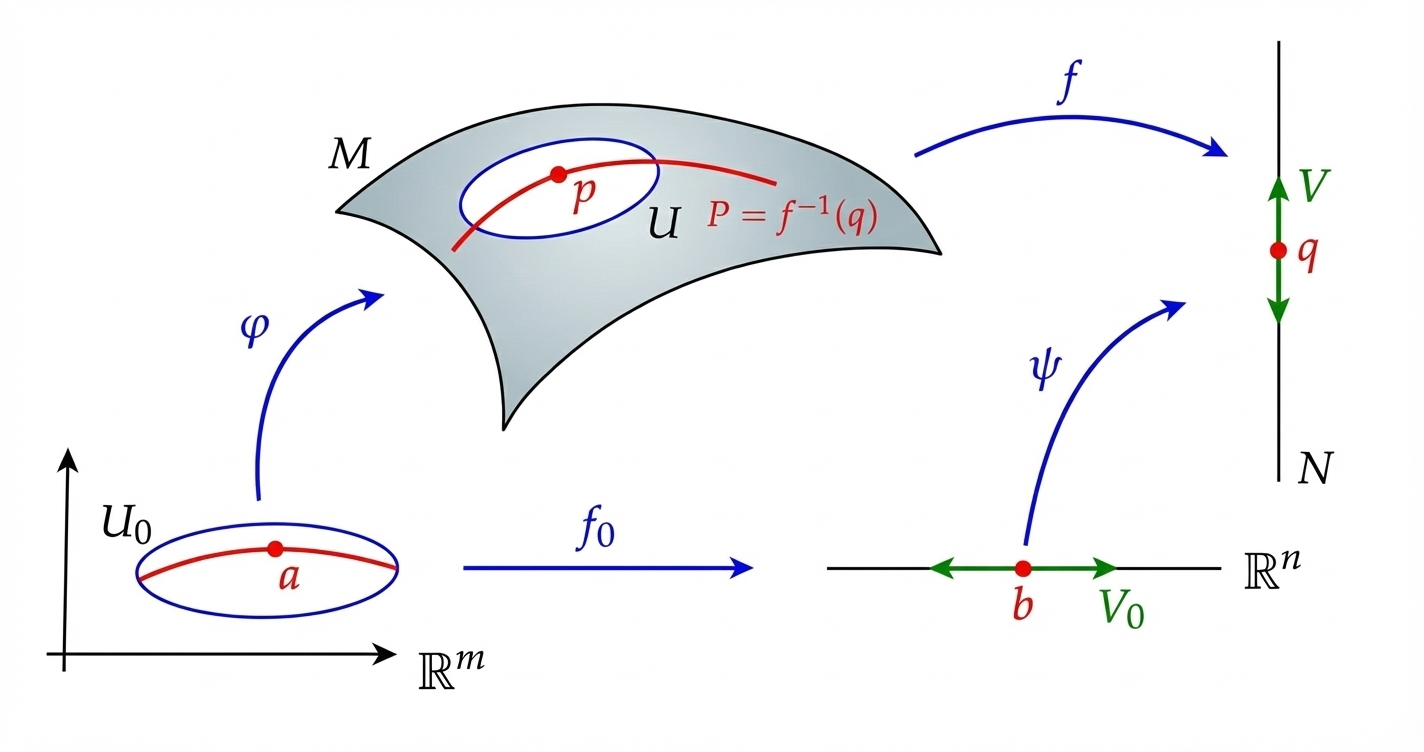
\includegraphics[width=0.7\textwidth, ]{Pictures/Th34.png}
		\label{fig:Th34}
\end{framed}
\end{figure}

	\vspace{-15pt}
	Пусть $b = \psi^{-1}(q)$. Если $a \in U_0$ удовлетворяет условию $f_0(a) = b$, то $\phi(a) = p \in U \cap P$. Отображения $d \phi_a : \R^m \to T_p M$, $d \psi^{-1}_q : T_q N \to \R^n$ сюръективны как изоморфизмы пространств, $df_p : T_p M \to T_q N$ сюръективно по условию,
	а значит, сюръективна и композиция этих линейных отображений, равная $d(f_0)_a : \R^m \to \R^n$ по цепному правилу. 
	Следовательно, точка $b$ является регулярным значением $f_0$. В частности, матрица Якоби функции 
	$f_0$ в точке $a$ имеет максимальный ранг $n$.
	По пункту (3) теоремы 3.1 $f_0^{-1}(b) = \{x \in U_0 : f(\phi(x)) = q\} = \phi^{-1}(U \cap P)$ является $(m-n)$-мерным многообразием в $\R^m$ (нули гладкой функции $f_0(x) - b$). 
	Найдем открытое $W \subset \R^{m-n}$ и параметризацию $\alpha : W \to \phi^{-1}(U \cap P)$ в окрестности $a$. 
	Теперь сузим $U_0$, и вместе с ним $U = \phi(U_0)$, тогда $\phi \circ \alpha : W \to U \cap P$ будет искомой параметризацией $P$ в окрестности точки $p$.
\end{myproof}



\begin{problem}
	Докажите, что в условиях теоремы $T_p P = \ker df_p$.
\end{problem}



\section{Экстремумы функций многих переменных}

\subsection{Локальные экстремумы}

\begin{definition}
	Пусть на открытом $U \subset \R^n$ задана функция $f : U \to \R$ и $a \in U$. 
	Точка $a$ называется \textit{точкой локального максимума} функции $f$, если 
	\[ \exists \delta > 0 \ \forall x \in \mathring{B_{\delta}}(a) : f(x) \leq f(a). \]
\end{definition}

\vspace{5pt}
Аналогично определяются точки локального минимума, точки строгого локального максимума и минимума. 
Все такие точки называются \textit{точками локального экстремума}. 

\begin{theorem}
	Если $a$ -- точка локального экстремума $f$ и $\exists \frac{\partial f}{\partial x_k}(a)$, то $\frac{\partial f}{\partial x_k}(a) = 0$.
\end{theorem}

\begin{myproof}
	Точка $a_k$ является точкой экстремума функции $\phi(t) = f(a_1, \dotsc, a_{k-1}, t, a_{k+1}, \dotsc, a_n)$.
	Так как $\phi$ дифференцируема в $a_k$ ($\phi'(a_k) = \frac{\partial f}{\partial x_k}(a)$), то по теореме Ферма $\phi'(a_k) = 0$.
\end{myproof}

\begin{corollary}
	Если $f$ дифференцируема в точке локального экстремума $a$, то ее дифференциал $df_a = 0$ (или $\nabla f(a) = 0$).
\end{corollary}

\begin{definition}
	Точка $a \in U$ называется \textit{стационарной} точкой функции $f$, если $f$ дифференцируема в $a$ и $df_a = 0$.
\end{definition}

\begin{reminder}
	Если $f \in C^2(U)$, то $d^2 f_a(h) = \sum \limits_{i, j = 1}^{n} \frac{\partial^2 f}{\partial x_i \partial x_j}(a) h_i h_j$ является квадратичной формой в $\R^n$ относительно компонент вектора $h \in \R^n$.
	Матрица данной квадратичной формы $H f(a) := \big( \frac{\partial^2 f}{\partial x_i \partial x_j}(a) \big)$ называется \textit{матрицей Гессе}, а определитель -- \textit{Гессианом}.
\end{reminder}

\begin{theorem}
	Пусть $U \subset \R^n$ открыто, $f \in C^2(U)$ и $a$ -- стационарная точка $f$. Тогда справедливы следующие утверждения:
	\begin{enumerate}[itemsep = 0pt, topsep = 5pt]
		\item Если $d^2 f_a(h) > 0$ при всех $h \neq 0$, то $a$ -- точка строгого локального минимума $f$,
		\item Если $d^2 f_a(h) < 0$ при всех $h \neq 0$, то $a$ -- точка строгого локального максимума $f$,
		\item Если существуют такие $h_+, h_- \in \R^n$, что $d^2 f_a(h_+) > 0$ и $d^2 f_a(h_-) < 0$, то $a$ не является точкой локального экстремума $f$.
	\end{enumerate}
\end{theorem}

\begin{myproof}
	Пусть $d^2 f_a (h) > 0$ при всех $h \neq 0$. Пользуясь тем, что $a$ стационарна, по формуле Тейлора с остаточным членом в форме Пеано при $h \neq 0$ имеем 
	\[ f(a+h) = f(a) + \frac12 d^2 f_a(h) + \alpha(h) |h|^2 = f(a) + |h|^2 \left( \frac12 d^2 f_a \left(\frac{h}{|h|}\right) + \alpha(h) \right), \]
	где $\alpha(h) \to 0$ при $h \to 0$. Поскольку функция $d^2 f_a$ непрерывна по $h$, а сфера $\{h \in \R^n : |h| = 1\}$ является компактом в $\R^n$, то по теореме 
	Вейерштрасса существует $m = \min \limits_{|h| = 1} d^2 f_a(h) > 0$. Выберем $\delta > 0$ так, что $|\alpha(h)| \leq m/4$ для всех $0 < |h| < \delta$. 
	Тогда $f(a+h) - f(a) \geq m/4 \cdot |h|^2 > 0$ для всех $h \in \mathring{B_{\delta}}(0)$, поэтому $a$ является точкой строгого минимума $f$.

	\vspace{5pt}
	Второй пункт сводится к первому заменой $f$ на $-f$.

	\vspace{5pt}
	В третьем пункте при достаточно малых $t$ по модулю по формуле Тейлора имеем
	\[ f(a+th_+) = f(a) + t^2 \left( \frac12 d^2 f_a(h_+) + \alpha(th_+) |h_+|^2 \right). \]
	Выражение в скобках при $t \to 0$ стремится к $\frac12 d^2 f_a (h_+) > 0$. Поэтому найдется такое $\delta_1 > 0$, что $f(a + th_+) - f(a) > 0$ при $0 < |t| < \delta$. 
	Аналогично находим $\delta_2 > 0 : f(a+th_-) - f(a) < 0$ при $0 < |t| < \delta_2$. Следовательно, выражение $f(x) - f(a)$ не сохраняет знак ни в какой окрестности $a$ и $f$ не имеет экстремума в точке $a$.
\end{myproof}

\begin{note}
	Если $d^2 f_a$ полуопределена, то теорема не позволяет сделать вывод о наличии экстремума в точке $a$. 
	Например, $O(0,0)$ является стационарной для $f = x^2 + y^4$, $g = x^2 - y^4$ и $d^2 f_O (h_1, h_2) = 2h_1^2 = d^2 g_O (h_1, h_2)$, при этом точка $O$ является точкой строгого минимума $f$ и не является точкой экстремума $g$.
\end{note}

\begin{note}
	Для исследования квадратичной формы на определенность можно привести ее к диагональному виду или использовать критерий Сильвестра.
\end{note}